% !TEX root = ../../main.tex
Часто за дослідними даними треба визначити, як залежить випадкова величина,
яку ми спостерігаємо, від однієї чи кількох інших випадкових величин.
Найзагальніший випадок --- \emph{статистична залежність}, як-от $\eta = \xi_1 + \xi_2$.
Є сенс розглядати математичне сподівання однієї величини при фіксованому значенні іншої (чи інших).
Наприклад, вартість квартири залежить від площі, поверху, району та багатьох інших параметрів,
але не є функцію (в звичному розумінні) від цих параметрів: якби функціональна залежність була,
то кожному набору цих параметрів відповідало б одне значення вартості --- у реальному світі такого не відбувається.
До того ж, врахувати всі можливі впливи на вартість квартири неможливо: площу чи поверх дізнатися просто,
але може статися, що продавець встановлює вартість на основі якихось власних міркувань, які <<зі сторони>> 
визначити чи оцінити неможливо.
Натомість, можна розглядати функціональну залежність середнього значення (математичного сподівання)
вартості від цих параметрів. Такий опис вже є більш реалістичним: хоча саме середнє значення спостерігати неможливо,
але можна збирати інформацію про значення вартості при різних значеннях деякого фіксованого набору параметрів.

\section{Математична модель лінійної регресії}
Нехай спостерігається деяка випадкова величина $\eta$, яка залежить від іншої випадкової
величини $\xi$ (або вектору $\vec{\xi}$), значення яких теж спостерігаються.
\begin{definition}
    Функція $f(x) = \E(\eta / \xi = x)$ (або $f(\vec{x}) = \E(\eta / \vec{\xi} = \vec{x})$)
    називається \emph{лінією регресії} $\eta$ на $\xi$ (або $\vec{\xi}$).
\end{definition}
Термін <<регресія>> вперше з'явився в роботі \href{https://uk.wikipedia.org/wiki/%D0%A4%D1%80%D0%B5%D0%BD%D1%81%D1%96%D1%81_%D0%93%D0%B0%D0%BB%D1%8C%D1%82%D0%BE%D0%BD}{Френсіса Гальтона} (англійського антрополога та статистика), який у 1885 році
досліджував зв'язок між зростом дітей та їх батьків. Виявилося, що в середньому діти високих батьків не були такими вже й високими, і навпаки.
Він назвав це \emph{<<регресією (поверненням) до посереднього>>}. Зокрема, Гальтон побудував таку лінію регресії (для зросту в дюймах):
\begin{gather*}
    \E\left(\text{зріст дитини}\middle/ \xi_1 = x\text{ (зріст батька)}, 
    \xi_2 = y\text{ (зріст матері)}\right) = 22.3 + 0.38 x + 0.28 y
\end{gather*}

\subsection{Однофакторна лінійна регресія}
Для початку будемо вважати, що $\eta$, яку називають \emph{вихідною величиною} або \emph{відкликом} залежить лише від однієї випадкової величини $\xi$,
яку називають \emph{вхідною} або \emph{фактором} чи \emph{предиктором}. Припустимо,
що було проведено $n$ експериментів зі значеннями фактору $\xi$ $x_1, x_2, ..., x_n$ та відповідними
значенням відклику $\eta$ $\eta_1, \eta_2, ..., \eta_n$. Позначимо
$\varepsilon_i = \eta_i - \E(\eta / \xi = x_i)$ --- це похибки спостережень, що дорівнюють різниці
між отриманим значенням та усередненим значенням $\eta$ при цьому значенні $\xi$.
Про розподіл $\vec{\varepsilon} = (\varepsilon_1, \varepsilon_2, ..., \varepsilon_n)^T$, як правило, мало що відомо:
припускається, що його координати незалежні, однаково розподілені, їх дисперсія невідома, але математичне сподівання нульове:
$\E\varepsilon_i = \E\eta_i - \E(\E(\eta / \xi = x_i)) = \E(\eta / \xi = x_i) - \E(\eta / \xi = x_i) = 0$.

Необхідно за значеннями $x_1, x_2, ..., x_n$ та $\eta_1, \eta_2, ..., \eta_n$ оцінити $f(x)$.
Величини $x_1, x_2, ..., x_n$ вважають невипадковими, тому вся випадковість зосереджена в
$\varepsilon_1, \varepsilon_2, ..., \varepsilon_n$ та $\eta_1, \eta_2, ..., \eta_n$.
Спочатку треба визначити вигляд цієї функції. Часто це випливає з постановки задачі або з'ясовується після візуалізації отриманих даних.
Якщо мова йде про \emph{лінійну регресію}, то вважають, що
$f(x) = \sum\limits_{k=1}^m \beta_k \psi_k(x)$, де $\psi_k(x)$ --- деякі функції, що називають \emph{базисними}.
Окремим часто застосованим випадком є \emph{поліноміальна регресія} з
$f(x) = \sum\limits_{k=0}^m \beta_k x^k$. Задача регресійного аналізу полягає в оцінці невідомих параметрів моделей наведеного виду.
\begin{remark}
    Назва <<лінійна регресія>> походить від того, що невідомі параметри $\beta_1, \beta_2, ..., \beta_n$ входять до $f(x)$ лінійно.
    Іноді (не зовсім коректно) вважається, що лінійною називають тільки ту модель, яка також
    є лінійною за $x$.
\end{remark}

\subsection{Метод найменших квадратів}
Оцінки $\vec{\beta} = (\beta_1, \beta_2, ..., \beta_m)^T$ можна знайти за допомогою методу максимальної правдоподібності,
застосованого до вектору $\eta = \left(\eta_1, \eta_2, ..., \eta_n\right)^T$.
Оскільки $\eta_i = \varepsilon_i + f(x_i)$, то розподіл $\eta_i$ буде таким самим, як 
$\varepsilon_i$, але з математичним сподіванням $f(x_i)$.

Припустимо, що $\vec{\varepsilon} \sim \mathrm{N}(\vec{0}, \sigma^2 \mathbb{I})$, де
$\mathbb{I}$ --- одинична матриця $n\times n$. Тоді
\begin{gather*}
    \mathcal{L}\left(\eta_1, \eta_2, ..., \eta_n, \vec{\beta}\right) = 
    \frac{1}{\left(\sqrt{2\pi} \sigma\right)^n} \exp\left\{
        -\frac{1}{2\sigma^2} \sum_{i=1}^n (\eta_i - f(x_i))^2
        \right\}
\end{gather*}
При фіксованому значенні $\sigma$ максимум функції правдоподібності по $\vec{\beta}$ досягається
при найменшому значенні $\sum\limits_{i=1}^n (\eta_i - f(x_i))^2 = \sum\limits_{i=1}^n \varepsilon_i^2$.
Цей окремий випадок ММП називається \emph{методом найменших квадратів (МНК)}.
\begin{definition}
    \emph{Оцінкою методу найменших квадратів (ОМНК)} для параметрів $\vec{\beta} = (\beta_1, \beta_2, ..., \beta_m)^T$
    називається такий набір цих параметрів, при яких досягається мінімум $\sum\limits_{i=1}^n \varepsilon_i^2$.
\end{definition}
Якщо ми знайдемо оцінки $\vec{\beta}^* = (\beta_1^*, \beta_2^*, ..., \beta_m^*)^T$,
то також знайдемо оцінку функції $f^*(x)$.
\begin{remark}
    На практиці іноді можуть припускати, що координати $\vec{\varepsilon}$ мають 
    розподіл Лапласа зі щільністю $f_\varepsilon(x) = \frac{\alpha}{2} e^{-\alpha|x|}$.
    В такому випадку знаходження максимуму функції правдоподібності зводиться
    до мінімізації суми $\sum\limits_{i=1}^n |\eta_i - f(x_i)|$ --- це вже не буде
    методом найменших квадратів.
\end{remark}
\begin{example}\label{intercept_fit}
    Нехай $f(x) = \beta$, тобто ми хочемо оцінити параметр лінії регресії, що є константою.
    Маємо $\eta_i = \beta + \varepsilon_i, \; i = 1,...,n$. По суті, ця задача є задачею оцінки невідомого математичного сподівання
    за вибіркою з незалежними й однаково розподіленими гауссівськими випадковими величинами
    $\eta_1, \eta_2, ..., \eta_n$. Знайдемо розв'язок задачі мінімізації
    $\sum\limits_{i=1}^n \varepsilon_i^2 = \sum\limits_{i=1}^n (\eta_i - \beta)^2 \to \min$:
    \begin{gather*}
        \frac{d}{d\beta} \left(\sum\limits_{i=1}^n (\eta_i - \beta)^2\right) = 
        - 2 \sum\limits_{i=1}^n (\eta_i - \beta) = 0 \Rightarrow \beta = \frac{1}{n} \sum\limits_{i=1}^n \eta_i \\
        \frac{d^2}{d\beta^2} \left(\sum\limits_{i=1}^n (\eta_i - \beta)^2\right) = 2n > 0
    \end{gather*}
    Отже, $\beta^* = \frac{1}{n}\sum\limits_{i=1}^n \eta_i = \overline{\eta}$. Такий само результат було
    отримано і при розв'язанні цієї задачі як задачі оцінки математичного сподівання.
\end{example}
\begin{exercise}
    Показати, що якщо координати вектора похибок $\varepsilon_i$ мають розподіл Лапласа, то максимізація
    такої функції правдоподібності буде еквівалентна мінімізації суми
    $\sum\limits_{i=1}^n |\eta_i - \beta|$, а розв'язком цієї задачі буде вибіркова медіана.
\end{exercise}

\subsection{Багатофакторна (множинна) лінійна регресія}
Тепер розглянемо випадок, коли $\eta$ залежить від $m$ факторів $\vec{\xi} = \left(\xi_1, \xi_2, ..., \xi_m\right)^T$.
\begin{definition}
    \emph{Простою лінійною багатофакторною регресійною моделлю} називається функція регресії
    вигляду
    $
        f(\vec{x}) = \E (\eta / \vec{\xi} = \vec{x}) = \beta_0 + \sum\limits_{i=1}^m \beta_i x_i
    $.
\end{definition}
Для спрощення цю модель іноді записують як $f(\vec{x}) = \sum\limits_{i=0}^m \beta_i x_i$, де фактор $x_0$ завжди
дорівнює 1. Надалі без втрати загальності будемо вважати, що розглядається модель
$f(\vec{x}) = \sum\limits_{i=1}^m \beta_i x_i$, в якій константного фактору або немає, або він присутній як один з факторів,
що завжди дорівнює $1$.

Нехай експеримент проводився $n$ разів, а на $j$-тому проведенні фактори набули значень
$\vec{x}^{(j)} = \left(x_1^{(j)}, x_2^{(j)}, ..., x_m^{(j)}\right)^T$, $j=1,...,n$. Як правило, $n > m$.
Також, після проведення $n$ експериментів маємо вектор відкликів
$\vec{\eta} = \left(\eta_1, \eta_2, ..., \eta_n\right)^T$, де
$\eta_j = f\left(\vec{x}^{(j)}\right) + \varepsilon_j = \sum\limits_{i=1}^m \beta_i x_i^{(j)} + \varepsilon_j$, $j=1,...,n$.
Цей вектор можна записати як $\vec{\eta} = F\vec{\beta} + \vec{\varepsilon}$, де
\begin{gather}
    F = \begin{pmatrix}
        x_1^{(1)} & x_2^{(1)} & \cdots & x_m^{(1)} \\
        x_1^{(2)} & x_2^{(2)} & \cdots & x_m^{(2)} \\
        \vdots & \vdots & \ddots & \vdots \\
        x_1^{(n)} & x_2^{(n)} & \cdots & x_m^{(n)} \\
    \end{pmatrix}
\end{gather}
Ця матриця називається \emph{матрицею плану}. Щоб знайти оцінку $\vec{\beta}$ за допомогою МНК,
зробимо \textbf{припущення}: $\mathrm{rang}{F} = m$ та $\vec{\varepsilon} \sim \mathrm{N}(\vec{0}, \sigma^2 \mathbb{I})$.
Перше припущення фактично означає, що фактори є лінійно незалежними, а друге --- що можна вимагати як незалежності похибок,
так і їх некорельованості. 
ОМНК для $\vec{\beta}$ буде розв'язком задачі мінімізації 
$$S(\beta) = \sum\limits_{i=1}^n \varepsilon_i^2 = \Vert\vec{{\varepsilon}}\Vert^2 = 
\Vert \vec{\eta} - F \vec{\beta} \Vert^2 \to \min$$
$S(\beta)$ --- це квадрат відстані від точки $\vec{\eta} \in \mathbb{R}^n$ (коректніше було б писати $\vec{\eta}_\text{зн}$,
але це ускладнить позначення) до точки $F\vec{\beta}$, що належить підпростору 
$L = \left\{F \vec{x} : \vec{x} \in \mathbb{R}^m \right\}$.
Мінімальною ця відстань буде тоді, коли вектор $\vec{\eta} - F\vec{\beta}$ буде ортогональним
до усіх векторів з $L$.
\begin{center}
    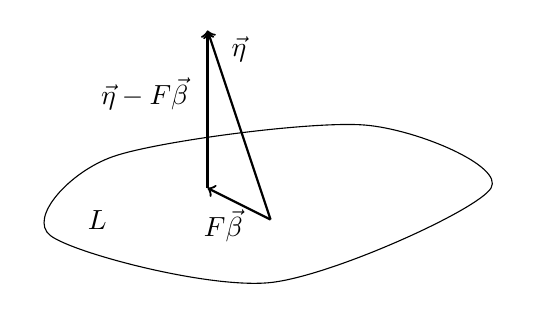
\begin{tikzpicture}
        \pgfmathsetmacro{\s}{4};
        \draw plot [smooth cycle] coordinates {(\s*0,\s*-0.15) (\s*0.7,\s*-0.3) (\s*1.4,\s*0) (\s*1,\s*0.2) (\s*0.2,\s*0.1)};
        \draw [thick, ->] (\s*0.5, \s*0) -- (\s*0.5, \s*0.5);
        \draw [thick, <-] (\s*0.5, \s*0) -- (\s*0.7, \s*-0.1);
        \draw [thick, ->] (\s*0.7, \s*-0.1) -- (\s*0.5, \s*0.5);
        \node at (\s*0.15, \s*-0.1) {$L$};
        \node at (\s*0.6, \s*0.44) {$\vec{\eta}$};
        \node [left] at (\s*0.47, \s*0.3) {$\vec{\eta} - F\vec{\beta}$};
        \node at (\s*0.55, \s*-0.12) {$F\vec{\beta}$};
    \end{tikzpicture}
\end{center}
Отже, $\forall\; \vec{x} \in \mathbb{R}^m: \left(F\vec{x}, \vec{\eta} - F \vec{\beta}\right) = 0$.
Оскільки $\left(F\vec{x}, \vec{\eta} - F \vec{\beta}\right) = \left(\vec{x}, F^T (\vec{\eta} - F \vec{\beta})\right)$,
то, з умови довільності $\vec{x}$ можна взяти, наприклад, вектори стандартного базису $\mathbb{R}^m$ та
отримати, що $F^T (\vec{\eta} - F \vec{\beta}) = 0 \Leftrightarrow F^T \vec{\eta} = F^T F \vec{\beta}$.
Умова $\mathrm{rang}{F} = m$ забезпечує існування $(F^T F)^{-1}$: нехай $\vec{x} \in \mathbb{R}^m$ та 
$F^T F \vec{x} = \vec{0}$, тоді $\vec{x}^T F^T F \vec{x} = (F\vec{x})^T F\vec{x} = \vec{0}$,
звідки $F\vec{x} = \vec{0}$, а з умови $\mathrm{rang}{F} = m$ маємо наслідок $\vec{x} = \vec{0}$,
тому $\mathrm{Ker} F^T F = \{ \vec{0}\}$.
Таким чином, отримуємо ОМНК для $\vec{\beta}$:
\begin{gather}\label{regr_coef}
    \vec{\beta}^* = (F^T F)^{-1} F^T \vec{\eta}
\end{gather}
Цю рівність іноді називають \emph{нормальним рівнянням}.
\begin{definition}
    Матрицю $A = F^T F$ називають \emph{інформаційною матрицею}, а $A^{-1} = 
    (F^T F)^{-1}$ --- \emph{дисперсійною матрицею (Фішера)}.
\end{definition}
Розглянемо властивості інформаційної матриці $A$:
\begin{enumerate}
    \item $F$ --- матриця розміру $n \times m$, $F^T$ --- розміру $m \times n$, тому
    $A$ --- квадратна матриця розміру $m \times m$.
    \item $A$ --- симетрична: $A^T = (F^T F)^T = F^T (F^T)^T = F^T F = A$.
    \item $A$ --- невід'ємно визначена: $\forall \; \vec{x} \in \mathbb{R}^m : \left(A\vec{x}, \vec{x}\right) = \left(F^T F \vec{x}, \vec{x}\right) = \left(F\vec{x}, F\vec{x}\right) = \Vert F \vec{x}\Vert^2 \geq 0$.
    \item Оскільки $A$ --- невід'ємно визначена та невироджена, то вона додатно визначена ($A > 0$) і тому $\exists! \; B > 0 :  B^2 = A$,
    тобто, існує і єдиний квадратний корінь $\sqrt{A}$.
\end{enumerate}
\begin{remark}
    Корінь із невід'ємно визначеної матриці будується за загальним принципом побудови функцій від симетричних матриць.
    Нехай $M$ --- невід'ємно визначена ($M \geq 0$) матриця $n \times n$, тоді її власні числа $\lambda_1 \geq \lambda_2 \geq ... \geq \lambda_n \geq 0$.
    Існує ортогональна матриця $U$, для якої $M = U \cdot \mathrm{diag}(\lambda_1, ..., \lambda_n) \cdot U^{-1}$.
    Для $S = U \cdot \mathrm{diag}(\sqrt{\lambda_1}, ..., \sqrt{\lambda_n}) \cdot U^{-1}$ маємо
    $S^2 = \left(\mathrm{diag}(\sqrt{\lambda_1}, ..., \sqrt{\lambda_n})\right)^2 = \mathrm{diag}(\lambda_1, ..., \lambda_n) = M$,
    причому $\sqrt{\lambda_1} \geq \sqrt{\lambda_2} \geq ... \geq \sqrt{\lambda_n} \geq 0$, тому $S \geq 0$. У випадку $M>0$
    мали б $\lambda_n > 0$, звідки $\sqrt{\lambda_n} > 0$ і $S > 0$. Зрозуміло, що $S = \sqrt{M}$ теж є симетричною матрицею. Також за побудовою
    $\sqrt{M}$ комутує з $M$ та $M^{-1}$ (якщо вона існує): $\sqrt{M} \cdot M = M \cdot \sqrt{M}$, $\sqrt{M} \cdot M^{-1} = M^{-1} \cdot \sqrt{M}$. 
\end{remark}
\begin{example}
    Знайти оцінки параметрів простої однофакторної лінійної регресійної моделі, що має вигляд $f(x) = \beta_0 + \beta_1 x$.
    Нехай є $n$ спостережень відклику $\vec{\eta}_\text{зн} = \left(y_1, y_2, ..., y_n\right)^T$ та
    фактора --- $\vec{\xi}_\text{зн} = \left(x_1, x_2, ..., x_n\right)$. Матрицю плану для спрощення можна записати з індексами $x_i$ замість $x^{(i)}$ як 
    $F = \begin{pmatrix}
        1 & x_1 \\
        \vdots & \vdots \\
        1 & x_n
    \end{pmatrix}$. Знайдемо дисперсійну матрицю:
    \begin{gather*}
        A = F^T F = \begin{pmatrix}
            1 & \cdots & 1 \\
            x_1 & \cdots & x_n
        \end{pmatrix} \cdot \begin{pmatrix}
            1 & x_1 \\
            \vdots & \vdots \\
            1 & x_n
        \end{pmatrix} = \begin{pmatrix}
            n & \sum\limits_{k=1}^n x_k \\
            \sum\limits_{k=1}^n x_k &  \sum\limits_{k=1}^n x_k^2
        \end{pmatrix} \\
        \det{A} = n \cdot \sum\limits_{k=1}^n x_k^2 - \left( \sum\limits_{k=1}^n x_k\right)^2 = 
        n^2 \cdot \left(\frac{1}{n}\sum\limits_{k=1}^n x_k^2 - 
        \left(\frac{1}{n} \sum\limits_{k=1}^n x_k\right)^2\right) = n^2 \cdot \left(\D^* \xi\right)_\text{зн} \\
        A^{-1} = (F^T F)^{-1} = \frac{1}{\det A} \begin{pmatrix}
            \sum\limits_{k=1}^n x_k^2 & - \sum\limits_{k=1}^n x_k \\
            - \sum\limits_{k=1}^n x_k & n
        \end{pmatrix} \\
        F^T \vec{\eta}_\text{зн} = \begin{pmatrix}
            1 & \cdots & 1 \\
            x_1 & \cdots & x_n
        \end{pmatrix} \cdot \begin{pmatrix}
            y_1 \\ \vdots \\ y_n
        \end{pmatrix} = \begin{pmatrix}
            \sum\limits_{k=1}^n y_k \\
            \sum\limits_{k=1}^n x_k y_k
        \end{pmatrix} \\
        \vec{\beta}^*_\text{зн} = (F^T F)^{-1} F^T\vec{\eta}_\text{зн} =
        \frac{1}{\det A} \begin{pmatrix}
            \sum\limits_{k=1}^n y_k \cdot \sum\limits_{k=1}^n x_k^2 - \sum\limits_{k=1}^n x_k \cdot \sum\limits_{k=1}^n x_k y_k \\
            - \sum\limits_{k=1}^n y_k \cdot \sum\limits_{k=1}^n x_k + n\cdot \sum\limits_{k=1}^n x_k y_k
        \end{pmatrix}
    \end{gather*}
    Якщо позначити $\sum\limits_{k=1}^n x_k = n\cdot \overline{x}$, $\sum\limits_{k=1}^n y_k = n\cdot \overline{y}$,
    $\sum\limits_{k=1}^n x_k y_k = n\cdot \overline{x y}$, $\sum\limits_{k=1}^n x_k^2 = n\cdot \overline{x^2}$, то
    \begin{gather*}
        \vec{\beta}^*_\text{зн} = \frac{1}{n^2 \cdot \left(\D^* \xi\right)_\text{зн}} \begin{pmatrix}
            n^2 \cdot \overline{y} \cdot \overline{x^2} - n^2 \cdot \overline{x} \cdot \overline{x y} \\
            - n^2 \overline{y} \cdot \overline{x} + n^2 \cdot \overline{x y}
        \end{pmatrix} = \frac{1}{\overline{x^2} - (\overline{x})^2} \begin{pmatrix}
            \overline{x^2} \cdot \overline{y} - \overline{x}\ \cdot \overline{xy} \\
            \overline{xy} - \overline{x} \cdot \overline{y}
        \end{pmatrix}
    \end{gather*}
    Зауважимо, що $\overline{xy} - \overline{x} \cdot \overline{y}$ --- це значення \emph{вибіркового аналогу коваріації} ${cov}(\xi, \eta)$, який ще можна позначити
    $\K^* \xi \eta$. Цей результат доволі очікуваний: якби статистична залежність між $\xi$ та $\eta$ описувалася рівнянням $\eta = \beta_0 + \beta_1 \xi$,
    то ${cov}(\xi, \eta) = {cov}(\xi, \beta_0 + \beta_1 \xi) = \beta_1 {cov}(\xi, \xi) = \beta_1 \D\xi$. 
\end{example}

\begin{remark}
    До простої лінійної багатофакторної моделі можна звести дослідження багатьох моделей більш загального виду.
    Наприклад, однофакторну модель виду $f(x) = \sum\limits_{k=1}^m \beta_k \psi_k(x)$
    можна розглядати як багатофакторну модель з факторами $x_k = \psi_k(x)$ (зокрема, це стосується поліноміальної регресії).
\end{remark}